%%
%% Author: dariochinelli
%% 2021-04-21
%%

\section{Potenziale nucleare}
Studiamo il potenziale nucleare considerando il nucleo del \emph{deuterio}, chiamato \emph{deutone}, composto da un protone ed un neutrone.

\paragraph{La Cromodinamica Quantistica (QCD)} è una teoria quantistica di campo e relativistica, è una teoria fondamentale che spiega l'interazione tra particelle elementari.
I nucleoni, i componenti del nucleo, protone e neutrone, sono a loro volta composti da \emph{quark}, i quali sono particelle elementari prive di dimensione e con carica frazionaria
\begin{itemize}
\item quark up $u$ ha carica $+\frac{2}{3}$
\item quark down $d$ ha carica $-\frac{1}{3}$
\end{itemize}
i nucleoni sono composti da 3 quark ciascuno e seguono la regola per cui
\begin{itemize}
\item il \textbf{protone} è composto da due quark \emph{up} ed un quark \emph{down}, ha quindi carica totale unitaria:
$$u+u+d = +\frac{2}{3} +\frac{2}{3} -\frac{1}{3} = 1$$
\item il \textbf{neutrone} è composto da due quark \emph{down} ed un quark \emph{up}, ha quindi carica totale nulla:
$$d+d+u = -\frac{1}{3} -\frac{1}{3} +\frac{2}{3} = 0$$
\end{itemize}
\begin{figure}[h]
\centering
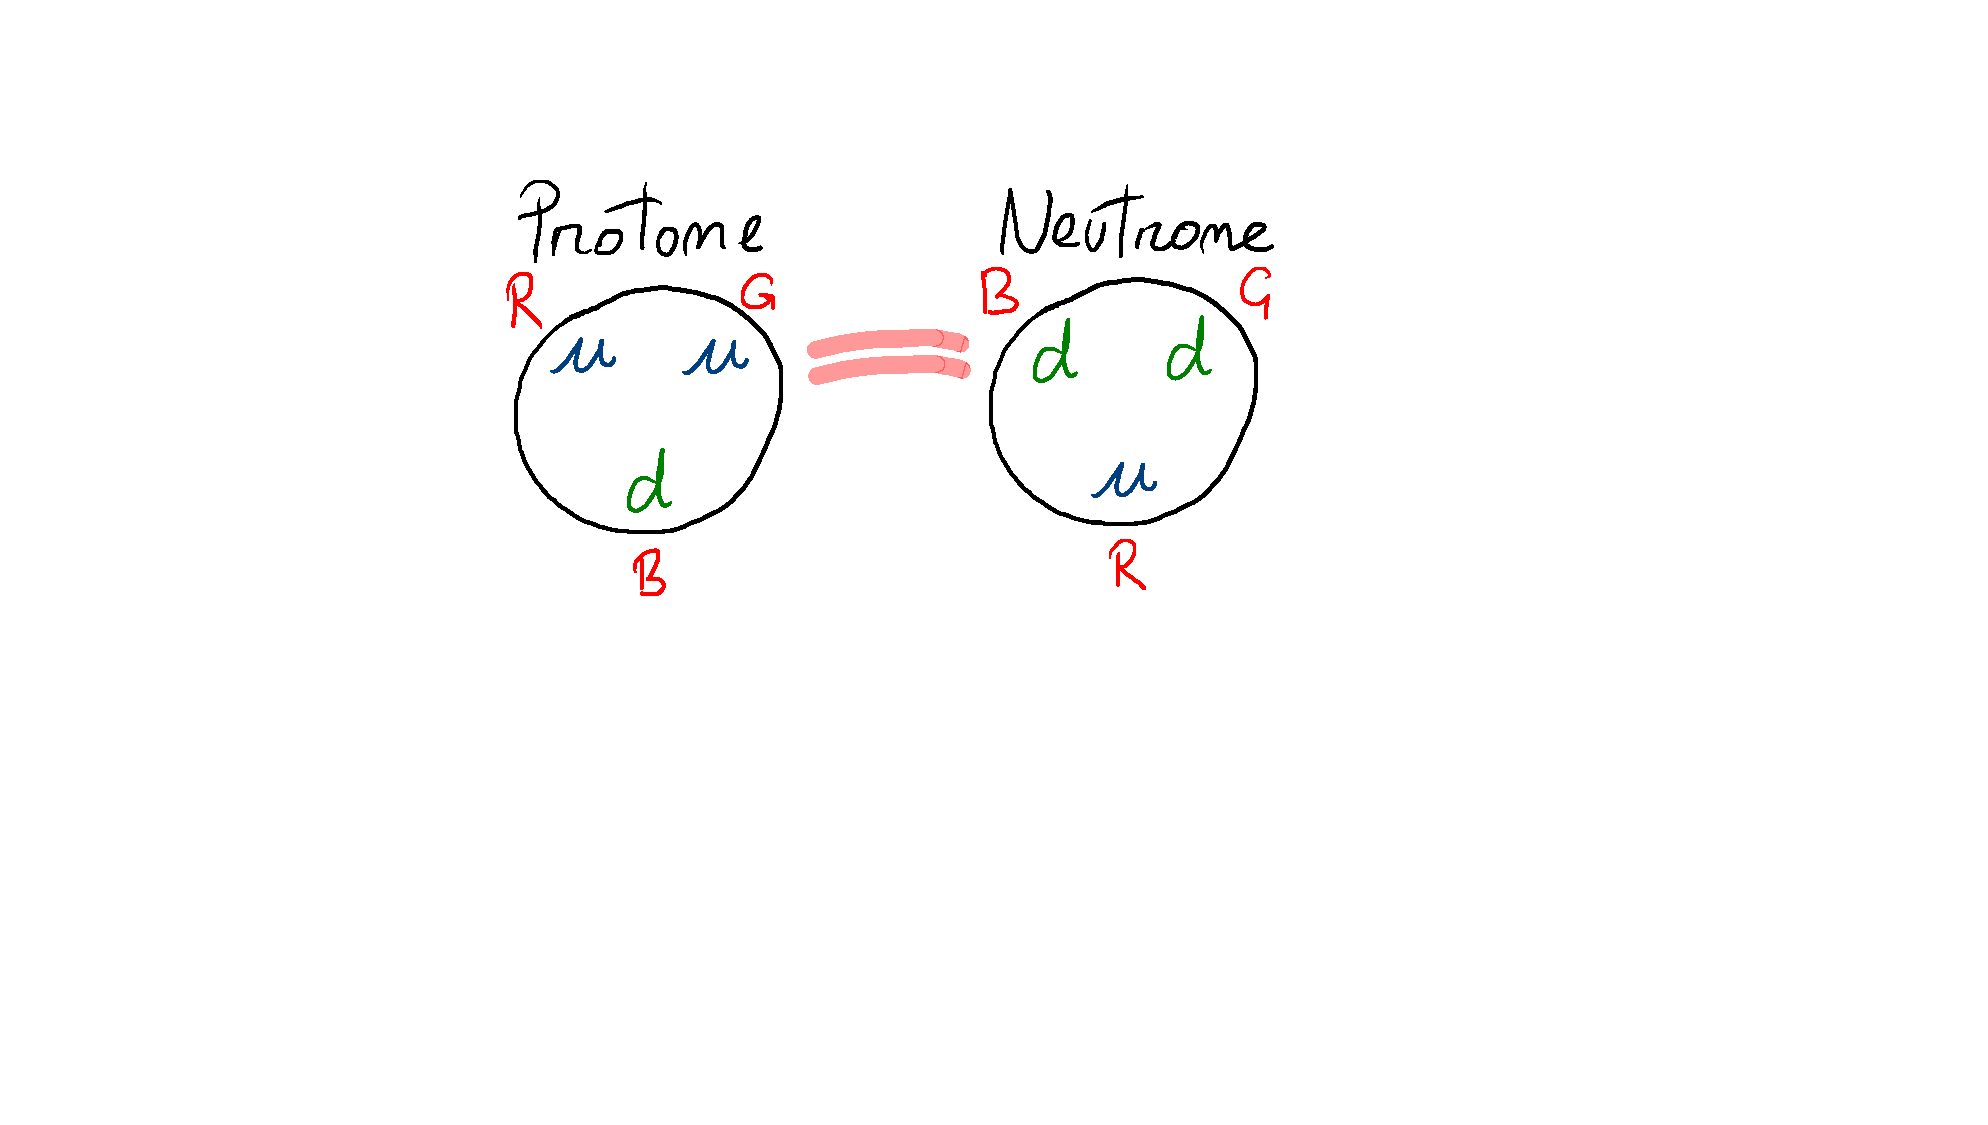
\includegraphics[scale=0.5]{/protone_neutrone_quark}
\caption{CAPTION}
\end{figure}

\paragraph{Carica di colore} I quark hanno anche un secondo tipo di carica: la \emph{carica di colore} che regola l'\emph{interazione forte} tra i quark.
La carica di colore può essere di tre tipi: Red (R), Green (G), Blue (B).
La somma delle tre cariche di colore dei rispettivi quark di un nucleone è nulla
\begin{equation}
R + G + B = 0
\end{equation}
un quark rosso (R) attira un quark verde (G) che attira un quark blu (B), mentre i quark dello stesso colore si respingono.
La teoria fondamentale della QCD esprime come l'interazione nucleare si possa interpretare come la carica di colore residua.



